\section{Notation and Preliminaries}

This section introduces the key terminology and notation used throughout the paper.

\subsection{Credit Exposure in DeFi Networks}

Let $X_G(q)$ be the set of tokens issued (or generated) by protocol $q$, and let $X_p(t)$ be the set of tokens held (or locked) by protocol $p$ at time $t$. We say that protocol $p$ has \emph{credit exposure} to protocol $q$ at time~$t$ if $p$ holds at least one token issued by $q$:
\begin{equation}
X_p(t)\cap X_G(q)\neq \varnothing.
\label{eq:credit-exposure-definition}
\end{equation}
Equivalently, $p$ is exposed to liabilities of $q$: if tokens issued by $q$ devalue or become illiquid, $p$ incurs losses. This token-mediated dependence generalises counterparty credit risk from traditional finance to DeFi, where exposures emerge through tokenised claims rather than explicit bilateral contracts. In practice, these dynamics can be tracked by reconstructing protocol-level TVL time series and monitoring how token composition changes over time \cite{wu2025dexposuredatasetbenchmarksinterprotocol}.

Figure~\ref{fig:exposure_example} shows how a single workflow can generate layered exposures. A user deposits ETH into Lido and receives stETH; stETH is wrapped into wstETH; wstETH is then deposited into Pendle, which splits it into PT-wstETH and YT-wstETH. On balance sheets, each step turns the upstream token into the downstream protocol's asset, so exposures stack: Pendle is exposed to the wstETH wrapper, which is exposed to Lido. If Lido suffers slashing or stETH de-pegs from ETH, losses can propagate through wstETH into Pendle and its PT/YT holders. This illustrates why DeFi exposures are naturally multi-layered and why DeXposure aims to measure them.

\begin{figure}[t]
    \centering
    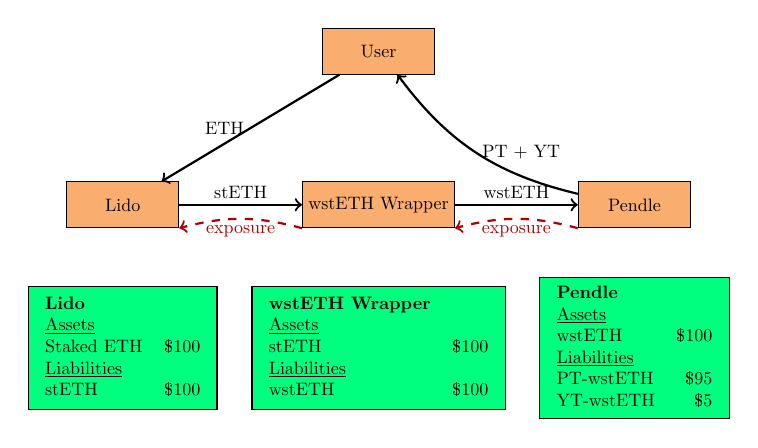
\begin{tikzpicture}[node distance=1.8cm, auto, scale=0.65, transform shape]
        \tikzstyle{entity} = [rectangle, draw, fill=Apricot, minimum width=2.2cm, minimum height=0.9cm, font=\normalsize]
        \tikzstyle{balance} = [rectangle, draw, fill=SpringGreen, minimum width=3.2cm, minimum height=2.4cm, font=\normalsize]
        \tikzstyle{exposure} = [->, thick, dashed, red!70!black]

        % User at top
        \node[entity] (user) at (0,3) {User};

        % Three protocols in a row
        \node[entity] (lido) at (-5,0) {Lido};
        \node[entity] (wrapper) at (0,0) {wstETH Wrapper};
        \node[entity] (pendle) at (5,0) {Pendle};

        % Balance sheets below each protocol
        \node[balance] (balanceLido) at (-5,-2.8) {
            \begin{tabular}{lr}
                \textbf{Lido} & \\
                \underline{Assets} & \\
                Staked ETH & \$100 \\
                \underline{Liabilities} & \\
                stETH & \$100
            \end{tabular}
        };
        \node[balance] (balanceWrapper) at (0,-2.8) {
            \begin{tabular}{lr}
                \textbf{wstETH Wrapper} & \\
                \underline{Assets} & \\
                stETH & \$100 \\
                \underline{Liabilities} & \\
                wstETH & \$100
            \end{tabular}
        };
        \node[balance] (balancePendle) at (5,-2.8) {
            \begin{tabular}{lr}
                \textbf{Pendle} & \\
                \underline{Assets} & \\
                wstETH & \$100 \\
                \underline{Liabilities} & \\
                PT-wstETH & \$95 \\
                YT-wstETH & \$5
            \end{tabular}
        };

        % Token flows (solid arrows)
        \draw[->, thick] (user) -- node[left, font=\normalsize] {ETH} (lido);
        \draw[->, thick] (lido) -- node[above, font=\normalsize] {stETH} (wrapper);
        \draw[->, thick] (wrapper) -- node[above, font=\normalsize] {wstETH} (pendle);
        \draw[->, thick] (pendle) to[bend left=20] node[right, font=\normalsize] {PT + YT} (user);

        % Credit exposure arrows (dashed red)
        \draw[exposure] (pendle.south west) to[bend right=15] node[below, font=\normalsize, text=red!70!black] {exposure} (wrapper.south east);
        \draw[exposure] (wrapper.south west) to[bend right=15] node[below, font=\normalsize, text=red!70!black] {exposure} (lido.south east);

    \end{tikzpicture}
    \caption{Multi-layer credit exposure in DeFi. A user stakes ETH with Lido, receiving stETH, which is wrapped into wstETH and deposited into Pendle. Each protocol holds the liability of the preceding one, creating a chain of credit exposures from Pendle to Lido.}
    \label{fig:exposure_example}
\end{figure}

\subsection{Mapping Tokens to Issuing Protocols}

To implement Eq.~\eqref{eq:credit-exposure-definition}, we must identify the issuing (or managing) protocol for each token. Let $\mathcal{P}$ be the set of protocols and $\mathcal{C}$ the set of blockchains. For any token $\sigma$ appearing in protocol $p$, a \emph{mapping function} $M(\sigma)$ returns the protocol $q$ that issues or governs $\sigma$. We construct $M$ via the following fallback pipeline:
\begin{enumerate}
  \item \emph{Metadata lookup:} match tokens to issuing protocols using DefiLlama metadata when available \cite{DefiLlama2026}.
  \item \emph{Manual mapping:} for high-TVL tokens without metadata links, assign issuers using documentation and expert judgment.
  \item \emph{Text-vector similarity:} otherwise, vectorise token and protocol descriptions using TF-IDF \cite{Qaiser2018} and assign $M(\sigma)$ as the most similar protocol, provided the cosine similarity exceeds a threshold $\theta$.
  \item \emph{Primary market tokens:} if no match is obtained, treat the token as its own protocol (e.g., WETH).
\end{enumerate}
This procedure attributes token movements to the appropriate issuer even when tokens are bridged or wrapped, and is used in curating DeXposure.

\subsection{Network Representation and Value Flows}

Over a discrete interval $\tau=t_2-t_1$, we represent exposures by a weighted directed graph $G_\tau=(P_\tau,E_\tau)$, where $P_\tau$ is the set of active protocols and $E_\tau$ the directed edge set. Each node $p\in P_\tau$ receives a \emph{node weight} equal to the value of its held assets at $t_2$:
\begin{equation}
w_\tau(p) = \sum_{\sigma\in X_p(t_1)\cap X_p(t_2)} v_{t_2,\sigma},
\label{eq:node-weight}
\end{equation}
where $v_{t_2,\sigma}$ is the USD value of token $\sigma$ at time $t_2$. Nodes below a threshold $\theta$ may be pruned.

To define the \emph{edge weight} from $p$ to $q$, we first compute token-level value flows:
\begin{equation}
F^{\sigma}_{p q,\tau} =
\begin{cases}
\max\bigl(0,\, -\Delta S^{\sigma}_{p,\tau}\bigr), & \text{if } \Delta S^{\sigma}_{p,\tau} < 0,\\
\max\bigl(0,\,\Delta S^{\sigma}_{q,\tau}\bigr), & \text{if } \Delta S^{\sigma}_{q,\tau} \ge 0,
\end{cases}
\label{eq:value-flow}
\end{equation}
where $\Delta S^{\sigma}_{p,\tau}=v_{p,t_2}^{\sigma}-v_{p,t_1}^{\sigma}$ is the change in the USD value of token $\sigma$ held by $p$ over $\tau$. Intuitively, if $p$ reduces holdings while $q$ increases holdings, $\sigma$ is interpreted as flowing from $p$ to $q$; the construction enforces non-negativity.

The \emph{edge weight} $w_\tau(e_{p q})$ aggregates flows over tokens mapped to issuer $q$:
\begin{equation}
w_\tau(e_{p q}) = \sum_{\sigma \in X_{p q, \tau}} F^{\sigma}_{p q,\tau},
\label{eq:edge-weight}
\end{equation}
where $X_{p q,\tau}$ is the set of tokens issued by $q$ that move from $p$ to $q$ over $\tau$. Positive $w_\tau(e_{p q})$ corresponds to increasing exposure from $p$ to $q$; for single-token protocols, that token's flow equals the edge weight. In summary, we compute $G_\tau$ by aggregating holdings at $t_1$ and $t_2$, assigning node weights, pruning small nodes, and summing positive token flows into issuer-specific edge weights. The resulting graph sequence captures the evolving credit-dependency structure curated in DeXposure.
